\begin{mainquestion}{rlhighpass}{RL High-Pass Filter Design}

Suppose you are tasked with attenuating a 60 Hz input component signal by a factor of 100 using an $RL$ high-pass circuit.

\begin{partquestion}{cornerfrequency}{What is the corner frequency $f_{c}$? How does this corner frequency relate to the time constant $\tau$ for an $RL$ circuit?}
\begin{answer}
We want the input to be reduced by a factor of 100, which in decibels is $-20\log 100 = -20(2) = -40\text{ dB}$. Using the asymptotic Bode approximation, the high-pass circuit will have a roll-off at $-20$ dB/decade from the corner frequency, so the corner frequency must be 2 decades above 60 Hz, namely:

\[
f_{c} = \left(60\text{ Hz}\right)\left(100\right) = 6\text{ kHz.}
\]

Since $\omega_{c} = 2\pi f_{c} = \frac{R}{L} = \frac{1}{\tau}$, it follows that:

\[
f_{c} = \frac{1}{2\pi\tau}.
\]
\end{answer}
\end{partquestion}

\begin{partquestion}{inductance}{You wish to design this circuit, and of course you have on hand a 17 k$\Omega$ resistor for the job. What is the necessary value of $L$?}
\begin{answer}
Since $2\pi f_{c} = \frac{R}{L}$, we can solve for $L$ and find:

\[
L = \frac{R}{2\pi f_{c}} = \frac{17\text{ k}\Omega}{2\pi\left(6\text{ kHz}\right)} = 0.451\text{ H.}
\]
\end{answer}
\end{partquestion}

\begin{partquestion}{bodeplots}{Draw the Bode plots (both magnitude and phase) of the transfer function $H\left(j\omega\right) = \frac{\mathbf{V_{\text{out}}}}{\mathbf{V_{\text{in}}}}$ for this high-pass filter.}
\begin{answer}
Since the transfer function of the high pass RL filter is:

\[
H\left(j\omega\right) = \frac{j\omega\frac{L}{R}}{1 + j\omega\frac{L}{R}} = \frac{1}{1 - \frac{j}{\omega}\frac{R}{L}}
\]

The Bode plots look as follows:

\begin{center}
    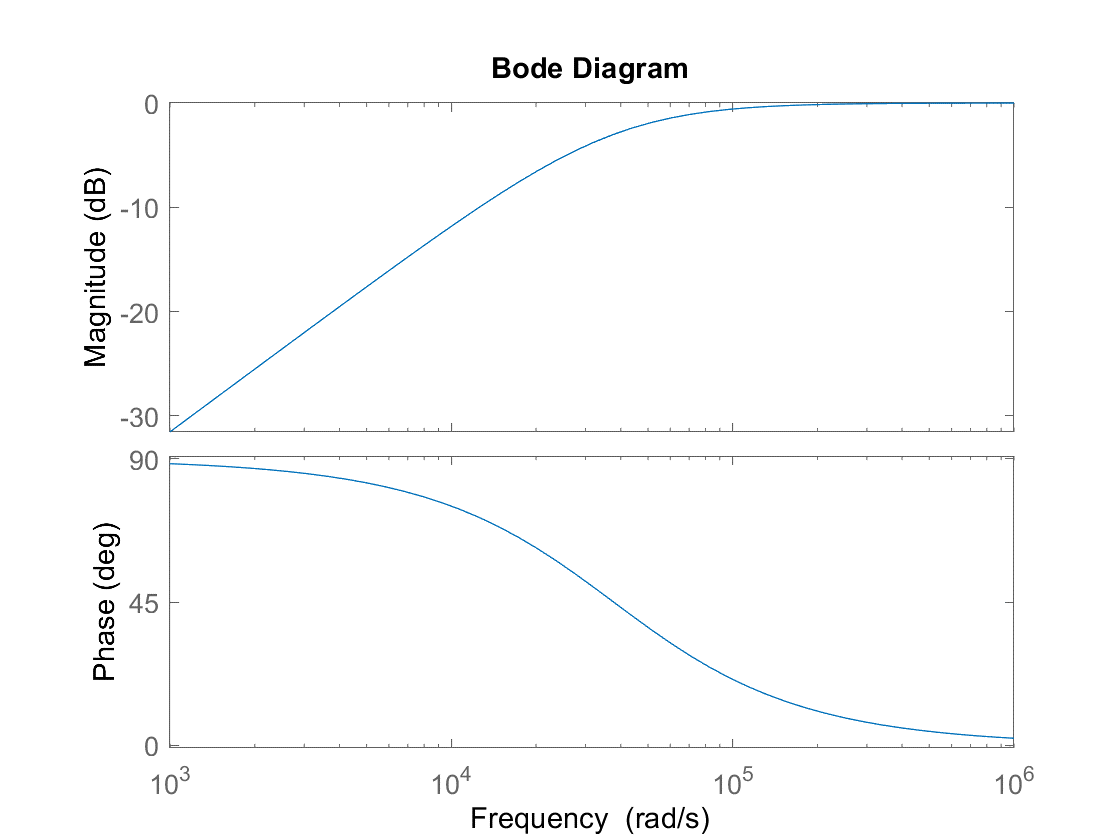
\includegraphics[width=5.65in]{questionbank/networks/rl_high_pass_design/v0/bode_plot.png}
\end{center}
\end{answer}
\end{partquestion}

\end{mainquestion}